\section{Auswertung}
\label{sec:Auswertung}
\subsection{Berechnung der Aktivierungsarbeit aus der Anlaufkurve}
Um die Aktivierungsarbeit der Dipole zu berechnen, werden die Messwerte für Temperatur und Strom
mit der Exponentialfunktion der Form
\begin{equation}
  y(T) = a\cdot e^{mT}
  \label{eqn:efit}
\end{equation}
gefittet.
% Mittlere heizspannung efit 3.2 0.13
\begin{figure}[H]
  \centering
  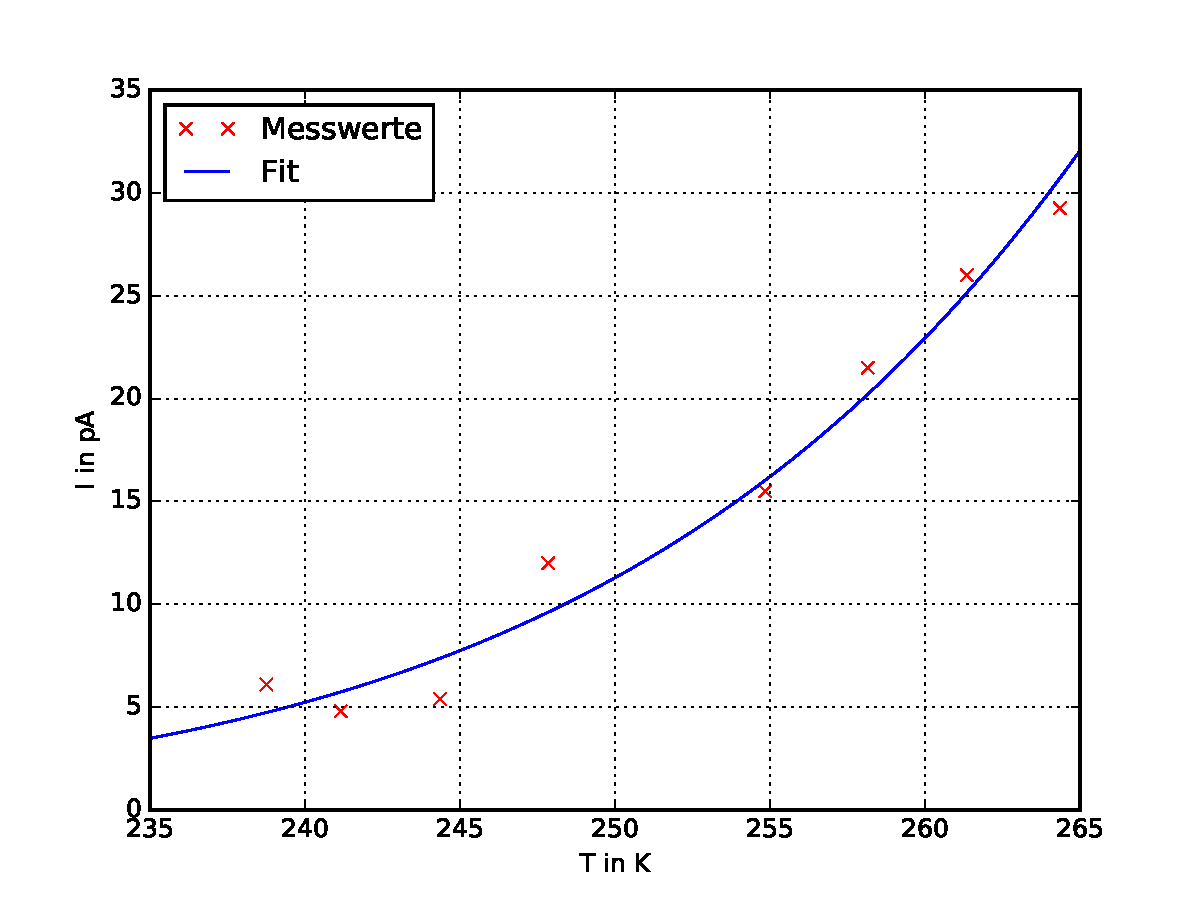
\includegraphics[width=0.8\textwidth]{plots/efit.pdf}
  \caption{Anlaufkurve des Depolarisationsstromes bei einer mittleren Heizrate von $H_1 =\SI{3.3 \pm 0.08}{\kelvin\per\minute}$.}
  \label{fig:efit1}
\end{figure}
\begin{figure}[H]
  \centering
  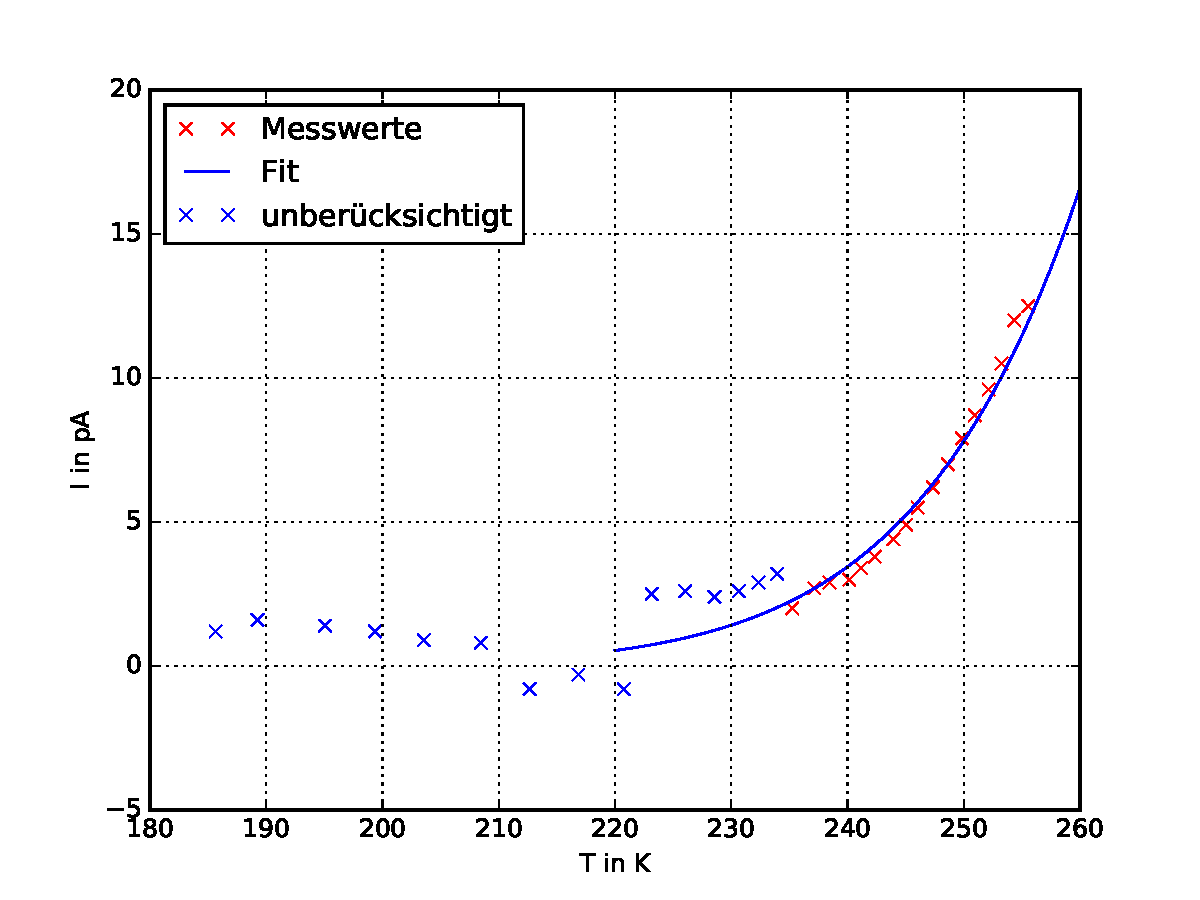
\includegraphics[width=0.8\textwidth]{plots/efit2.pdf}
  \caption{Anlaufkurve des Depolarisationsstromes bei einer mittleren Heizrate von $H_2 =\SI{1.26 \pm 0.07 }{\kelvin\per\minute}$}
  \label{fig:efit2}
\end{figure}
Die gefitteten Anlaufkurven sind in Abbildung \ref{fig:efit1} und \ref{fig:efit2} zu sehen.
Für den Fit der zweiten Messung wurden die in Abbildung \ref{fig:efit2} gezeigten bauen Messwerte nicht berücksichtigt.
Aus den angehängten Messwerten wurden ausserdem mittlere Heizraten für beide Messungen bestimmt. Die aus den Werten der Anlaufkurve ermittelten Heizraten lauten:
\begin{center}
  $H_1 =(3.2 \pm 0.13)\frac{\symup{K}}{\text{min}}$, $H_2 = (1.26 \pm 0.064)\frac{\symup{K}}{\text{min}}$
\end{center}
Aus der Ausgleichsrechnung ergeben sich die Fitparameter zu
\begin{center}
    $m_1 = 5680.23$, $ a_1= 24.98$, $m_2 = 5425.56$, $a_2 = 23.87$.
\end{center}
Aus dem Fitparameter $m_{(1/2)}$ werden dann nach
\begin{equation}
  W_{1/2} = m_{1/2}\cdot k_B
\end{equation}
die Austrittsarbeiten berechnet. Die berechneten Arbeiten lauten:
\begin{center}
  $W_1 = \SI{78}{\zepto\joule}$ und $W_2 = \SI{75}{\zepto\joule}$
\end{center}
\subsection{Berechnung der Aktivierungsenergie durch Integrieren}

%Die mittleren Relaxationszeiten der Probe wurden durch \eqref{eqn:tau2} unter Zuhilfenahme riemannscher Integration, durchgeführt mittels Python \cite{Python}, berechnet und in Abb. \ref{fig:integral} dargestellt, sowie in Tab. \ref{tab:tau} angegeben. Hierbei wurde der zweite Anstieg jeweils nicht betrachtet.
%\begin{table}
%  \centering
%  \caption{Aus Messwerten bestimmte mittlere Lebensdauern $\tau(T)$}
%  \sisetup{round-mode=places, round-precision= 0, scientific-notation= fixed, fixed-exponent = 0}
%  \begin{tabular}{|S[round-precision = 2]|S|S[round-precision = 2]|S|}
%    \toprule
%    {$\tau_1$} & {$T_1$} & {$\tau_2$} & {$T_2$} \\
%    \midrule
%    1.908740956591639815e+03 & 2.387499999999999716e+02 & 3.522600151171581274e+03 & 2.401499999999999773e+02\\
%    2.362137957317072505e+03 & 2.411499999999999773e+02 & 3.080751173708920760e+03 & 2.411499999999999773e+02\\
%    2.048644701086956047e+03 & 2.443499999999999659e+02 & 2.714526823387584500e+03 & 2.423499999999999659e+02\\
%    8.852892945544554095e+02 & 2.478499999999999659e+02 & 2.285400313971741980e+03 & 2.439499999999999886e+02\\
%    5.703757202304738030e+02 & 2.548499999999999659e+02 & 2.009335219236209241e+03 & 2.450499999999999829e+02\\
%    3.587953862164661700e+02 & 2.581499999999999773e+02 & 1.750863885377159932e+03 & 2.460499999999999829e+02\\
%    2.421499330015314513e+02 & 2.613499999999999659e+02 & 1.499362579677541362e+03 & 2.473499999999999659e+02\\
%    1.622165474974464132e+02 & 2.643499999999999659e+02 & 1.273160173160173599e+03 & 2.486499999999999773e+02\\
%    1.170913993362832315e+02 & 2.673499999999999659e+02 & 1.076870748299320212e+03 & 2.498499999999999659e+02\\
%    9.322714597478157827e+01 & 2.701499999999999773e+02 & 9.295130481571159180e+02 & 2.509499999999999886e+02\\
%    7.279322687224697574e+01 & 2.730499999999999545e+02 & 7.892063492063492731e+02 & 2.521499999999999773e+02\\
%5    4.432711693548425558e+01 & 2.755499999999999545e+02 & 6.723451822043375614e+02 & 2.532499999999999716e+02\\
%    &  & 5.401920438957482702e+02 & 2.543499999999999659e+02\\
%     &  & 4.628270280444191940e+02 & 2.555499999999999829e+02\\
%     &  & 4.199698851872760770e+02 & 2.564499999999999886e+02\\
%     &  & 3.789339604154420158e+02 & 2.576499999999999773e+02\\
%     &  & 3.752554903239846453e+02 & 2.585499999999999545e+02\\
%%     &  & 3.430132708821246297e+02 & 2.605499999999999545e+02\\
%     &  & 3.189200680272110731e+02 & 2.616499999999999773e+02\\
%     &  & 3.213481338481335570e+02 & 2.624499999999999886e+02\\
%     &  & 3.253534226190483878e+02 & 2.633499999999999659e+02\\
%     &  & 3.228402865570999438e+02 & 2.642500000000000000e+02\\
%     &  & 3.500768049155159929e+02 & 2.650499999999999545e+02\\
%5    &  & 3.417670682730939120e+02 & 2.660499999999999545e+02\\
%%     &  & 2.476190476190470235e+02 & 2.687500000000000000e+02\\
%     &  & 1.904761904761904532e+02 & 2.699499999999999886e+02\\
%     &  & 1.380952380952397220e+02 & 2.710499999999999545e+02\\
%     & & 9.523809523809522659e+01 & 2.719499999999999886e+02\\
%     & & 4.761904761904761330e+01 & 2.729499999999999886e+02\\
%     \bottomrule
%  \end{tabular}
%  \label{tab:tau}

%\end{table}
%\begin{figure}
%  \centering
%  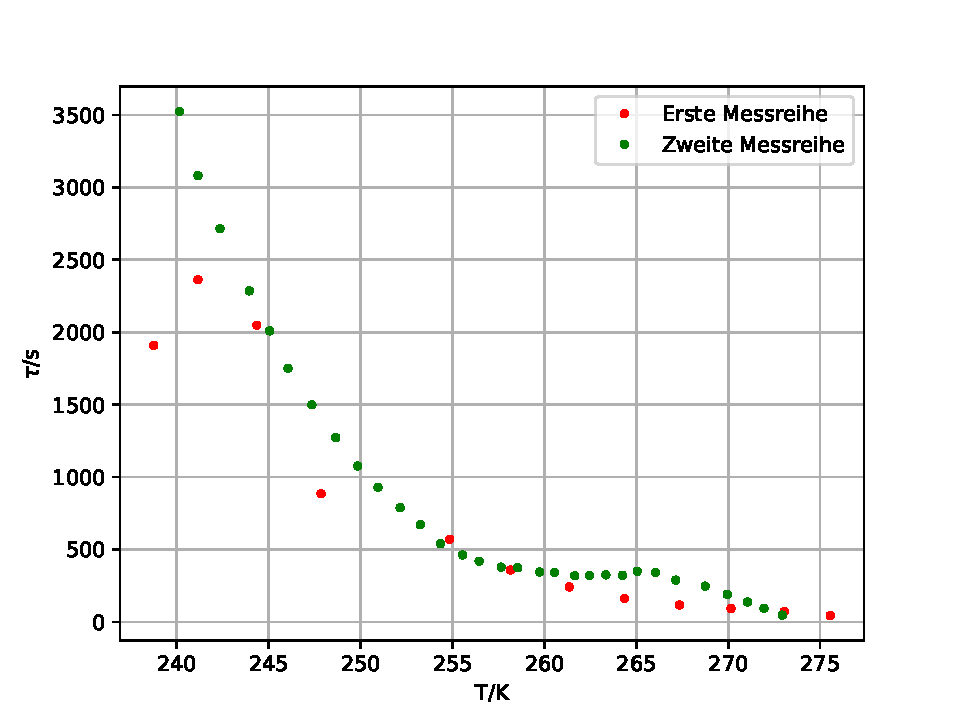
\includegraphics{./plots/integral.pdf}
%  \caption{Mittlere Lebensdauern $\tau(T)$ der Probe in Abhängigkeit der Temperatur $T$, entnommen aus Tab. \ref{tab:tau}.}
%  \label{fig:integral}
%\end{figure}

Eine lineare Ausgleichsrechnung von $\ln(\frac{\int_{T}^{\infty}i(T')\symup{d}T'}{i(T)})$ augetragen gegen $1/T$ (siehe Abb. \ref{fig:log}) liefert
\begin{center}
  $m_1 = \SI{7417 \pm 426}{\kelvin}$ und $b_1 = -25.5\pm1.6$
\end{center}
für die erste Messung. $m$ bezeichnet hierbei die Steigung der Geraden, $b$ den Ordonatenabschnitt.
Es ergibt sich hierdurch
\begin{equation*}
  W_1^i = k_b m_1 = \SI{102 \pm 6}{\zepto\joule}.
\end{equation*}

\begin{figure}
  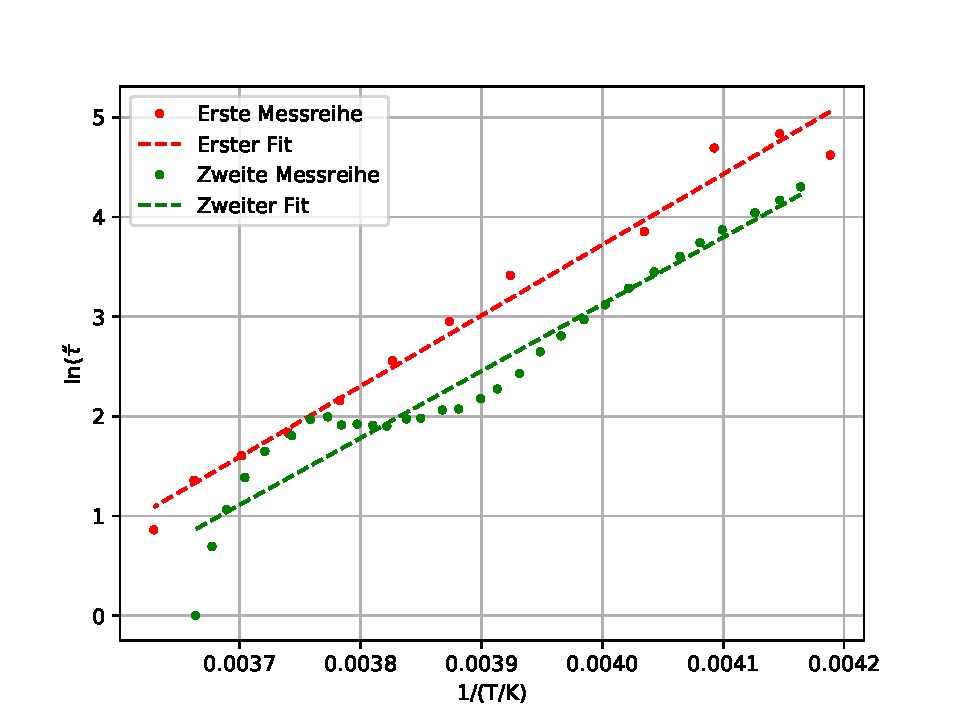
\includegraphics{./plots/log.pdf}
  \caption{}
  \label{fig:log}
\end{figure}

Für die zweite Messreihe ergibt sich entsprechend:
\begin{center}
  $m_2 =  \SI{6713 \pm 324}{\kelvin}$, $b_2=-23.7 \pm 1.3$, $W_2^i= \SI{93 \pm 4}{\zepto\joule}$
\end{center}

\subsection{Bestimmung der charakteristischen Relaxationszeit}
Als Maxima wurden gewählt:
\begin{center}
  $T_{max,1} = \SI{-8.8}{\celsius}$ und $T_{max,2} = \SI{-16.7}{\celsius}$
\end{center}
Nach Verrechnung dieser Werte, sowie $W_1$ bzw. $W_2$, ergibt sich gemäß \eqref{eqn:tau3}:
\begin{center}
  $\tau_{max,1}=  \SI{177\pm 10}{\second}$ und $\tau_{max,2}=  \SI{466\pm23}{\second}$
\end{center}

Dieser Werte lassen sich wiederrum durch \eqref{eqn:relaxation} in $\tau_0$ überführen.
Dies liefert
\begin{center}
  $\tau_{0,1}= \SI{0.12 \pm 0.19}{\nano\second}$ und $\tau_{0,2} = \SI{2.0 \pm 2.6}{\nano\second}$.
\end{center}
